\chapter{物理命中、回避、会心与反击}

\section{普通回避的源码判定顺序}

源码中物理攻击的判定顺序为：先检查防守方是否具备\emph{根本不能闪}的条件,再进入普通回避主体。”回避率”分为三层：硬性失败条件、独立前判、普通回避公式本身。

普通回避的硬性失败条件包括：当前动作是 \code{BATTLE\_COM\_GUARD}\footnote{\code{gmsv/src/battle/battle.c}, 第2847行。}、存在吸收/反射/消失类伤害反应、当前无法行动且不满足”集气但未被天罗地网或盾击限制”的例外、挂有 \code{CHAR\_BATTLEFLG\_NODUCK}，以及特殊战斗标记。这些条件一旦命中,后续不再进入普通回避公式。

若编译启用 \code{_PETSKILL\_SETDUCK}\footnote{\code{gmsv/src/include/version.h}, 第287行。},防守方可能在普通回避前先经过额外回避前判。该前判读取 \code{CHAR\_MYSKILLDUCK} (剩余回合) 与 \code{CHAR\_MYSKILLDUCKPOWER} (前判成功率)。

\begin{theorem}[回避前判与普通回避的复合]
\label{thm:duck-front-composite}
设前判成功率为 $p_{\mathrm{front}}$,普通回避主体成功率为 $p_{\mathrm{normal}}$,则总闪避率为
\begin{equation}
    p_{\mathrm{total}} = p_{\mathrm{front}} + \bigl(1-p_{\mathrm{front}}\bigr)p_{\mathrm{normal}}.
\end{equation}
\end{theorem}

\begin{proof}
前判失败概率为 $1-p_{\mathrm{front}}$,此时进入普通回避,成功率为 $p_{\mathrm{normal}}$。两阶段独立,总成功率为前判成功加前判失败后普通回避成功。
\end{proof}

\begin{remark}
职业技能 \textbf{回避} 不是独立前判。\code{CHAR\_WORK\_P\_DUCK} 仅为”启用倍率”标记,\code{CHAR\_WORKMOD\_P\_DUCK} 为倍率值；两者将已算出的普通回避值乘以比例,属于普通回避主体的后段修正。
\end{remark}

\section{命中与回避的源码公式}

\subsection{身份修正与主判定顺序}

设攻击方与防守方原始固定敏分别为 $\attdex$ 与 $\defdex$。进入普通回避主体前,源码按攻守身份做\emph{单边修正}\footnote{\code{gmsv/src/battle/battle.c}, 第2865-2890行。},而非对两边同时缩放。记修正后的固定敏为 $\widetilde{\attdex}$ 与 $\widetilde{\defdex}$,则在当前主分支下可整理为
\begin{equation}
    (\widetilde{\attdex},\widetilde{\defdex})=
    \begin{cases}
        (\lfloor 0.8\attdex \rfloor,\defdex), & \text{敌人打宠物}, \\
        (\attdex,\lfloor 0.8\defdex \rfloor), & \text{非敌人打宠物}, \\
        (\lfloor 0.6\attdex \rfloor,\defdex), & \text{非玩家打玩家}, \\
        (\attdex,\lfloor 0.6\defdex \rfloor), & \text{玩家打非玩家}, \\
        (\attdex,\defdex), & \text{其余情形}.
    \end{cases}
\end{equation}
所有取整来自源码将浮点乘法结果回写到整型变量的截断。

令
\begin{equation}
    B = \max\{\widetilde{\attdex},\widetilde{\defdex}\}, \qquad S = \min\{\widetilde{\attdex},\widetilde{\defdex}\},
\end{equation}
并定义比例项
\begin{equation}
    w = \begin{cases}
        1, & \widetilde{\defdex} \ge \widetilde{\attdex}, \\
        \dfrac{\widetilde{\defdex}}{\widetilde{\attdex}}, & \widetilde{\defdex} < \widetilde{\attdex}.
    \end{cases}
\end{equation}
再定义动作参数
\begin{equation}
    \alpha = \begin{cases}
        0.027, & \text{若防守方当前动作是 \code{BATTLE\_COM\_JYUJYUTU}（咒术）}, \\
        0.02, & \text{否则}.
    \end{cases}
\end{equation}
则普通回避主体的核心基础值为
\begin{equation}
    d_{\mathrm{core}} = \sqrt{\max\!\left\{\frac{B-S}{\alpha},0\right\}}\,w.
\end{equation}

在此之后，源码按如下顺序继续叠加或修正：
\begin{equation}
    d_{\mathrm{pre}} = d_{\mathrm{core}} + L_d + M + R_{\mathrm{drunk}} + 40I_{\mathrm{bow}} + N,
\end{equation}
\begin{equation}
    u_0 = \operatorname{clip}_{[1,7500]}\!\bigl(100d_{\mathrm{pre}}\bigr),
\end{equation}
\begin{equation}
    u_1 = \max\{0, u_0 - R_{\mathrm{hit}}\},
\end{equation}
\begin{equation}
    u_2 = \left\lfloor \frac{u_1(100+P)}{100} \right\rfloor,
\end{equation}
\begin{equation}
    u_3 = \begin{cases}
        1.4u_2, & \text{若攻击方当前使用混乱攻击}, \\
        u_2, & \text{否则}.
    \end{cases}
\end{equation}
最终以 \code{RAND(1,10000) <= u3}\footnote{\code{gmsv/src/battle/battle.c}, 第2923行。} 判定是否闪避成功。这里 $L_d$ 表示防守方幸运；$M$ 表示全局回避修正 \code{gBattleDuckModyfy}；$R_{\mathrm{drunk}}$ 表示攻击方醉酒时附加的 \code{RAND(20,30)}，否则取 $0$；$I_{\mathrm{bow}}$ 为攻击方是否持弓的指示量，源码该分支额外加两次 $20$；$N$ 表示 \code{BATTLE\_COM\_S\_NOGUARD} 带来的技能附加值；$R_{\mathrm{hit}}$ 表示 \code{AddHit} 在后段扣掉的命中修正；$P$ 表示职业技能 \textbf{回避} 的倍率加成。


\subsection{咒术动作分支与职业技能是否共用回避链}

从源码命名与分支用途看,\code{BATTLE\_COM\_JYUJYUTU}\footnote{\code{gmsv/src/include/battle.h}, 第45行。} 译作”\textbf{咒术动作分支}”。该常量名对应日文”咒术”的罗马字写法；现代常见拼写为 \emph{jujutsu},源码保留较旧的 \code{JYUJYUTU} 形式。式~\eqref{eq:dodge-base} 中 $\alpha=0.027$ 的触发条件仅看\emph{防守方当前动作}是否为 \code{BATTLE\_COM\_JYUJYUTU},不看攻击方是否使用职业技能。

职业技能下达动作时统一写入各自的 \code{BATTLE\_COM\_S\_*},不直接标记为 \code{BATTLE\_COM\_JYUJYUTU}。”使用职业技能”与”进入咒术回避参数分支”不是同一件事。需要区分的是：该职业技能后续是否仍调用普通物理攻击序列 \code{BATTLE\_AttackSeq()}\footnote{\code{gmsv/src/battle/battle.c}, 第1847行。},从而继续进入 \code{BATTLE\_DuckCheck()}\footnote{\code{gmsv/src/battle/battle.c}, 第2847行。}。若是,则仍受”目标当前动作是 \code{BATTLE\_COM\_JYUJYUTU}”影响；若否,则不按本章的普通物理回避链解释。表~\ref{tab:profession-dodge-paths} 汇总当前源码下的关键分类。

\begin{table}[H]
    \centering
    \caption{职业技能与普通物理回避链的关系}
    \label{tab:profession-dodge-paths}
    \begin{tabularx}{\textwidth}{>{\raggedright\arraybackslash}p{2.7cm} >{\raggedright\arraybackslash}p{3.8cm} >{\raggedright\arraybackslash}p{3.8cm} >{\centering\arraybackslash}p{1.8cm} X}
        \toprule
        技能类别 & 代表技能 & 主要结算入口 & 调用 \code{BATTLE\_DuckCheck} & 是否受目标 \code{JYUJYUTU} 的 $0.027$ 影响 \\
        \midrule
        直接物理职业攻击 & 爆裂、连环攻击、双重攻击、骑宠攻击、舍命攻击、弱点攻击、掠夺、混乱攻击 & \code{battle\_profession\_attack\_fun()} $\rightarrow$ \code{BATTLE\_AttackSeq()} & 是 & 是；但触发前提仍是\emph{目标当前动作}为 \code{BATTLE\_COM\_JYUJYUTU} \\
        带物理命中判定的状态攻击 & 盾击、剧毒武器 & \code{battle\_profession\_status\_chang\_fun()} $\rightarrow$ \code{BATTLE\_AttackSeq()} & 是 & 是；逻辑与直接物理职业攻击相同 \\
        辅助与自我强化技能 & 专注战斗、回避、回复、舍己为人、激怒、能量聚集、陷阱、驯化等 & \code{battle\_profession\_assist\_fun()} & 否 & 否；不按普通物理回避链处理 \\
        法师攻击技能 & 火球、冰箭、火枪、雷击、末日、血蛊等 & \code{battle\_profession\_attack\_magic\_fun()} $\rightarrow$ \code{PROFESSION\_MAGIC\_ATTAIC()} & 否 & 否；应按职业法术命中链分析 \\
        主分发归入法术攻击组的特殊技能 & 穿透攻击、缠绕攻击 & 当前主分发进入职业法术攻击组 & 本文暂不按普通物理回避链归类 & 本文暂不把它们并入 $\alpha=0.027$ 的普通物理回避分析，留待后续校核 \\
        \bottomrule
    \end{tabularx}
\end{table}

表~\ref{tab:profession-dodge-paths} 的含义可压缩为：\textbf{职业技能不因”职业技能”身份自动进入 \code{BATTLE\_COM\_JYUJYUTU} 分支；仅那些后续仍调用普通物理回避函数的职业技能,才会在目标当前动作恰好是咒术分支时,间接受到 $\alpha=0.027$ 的影响。}

\subsection{PVP 内部的人宠对象组合差异}

即使在玩家对玩家战斗中,\emph{人打人、人打宠、宠打人、宠打宠} 也不能共用同一简化公式。源码先按攻击侧与防守侧的单位类型进入不同分支,再决定缩放哪一边的固定敏,以及是否切到线性口径。表~\ref{tab:pvp-pairings} 汇总当前源码下三类物理概率机制在 PVP 内部的对象组合差异。这里”人”指玩家本体,”宠”指玩家宠物。

\begin{table}[H]
    \centering
    \caption{PVP 中不同攻守对象组合的概率口径差异}
    \label{tab:pvp-pairings}
    \begin{tabularx}{\textwidth}{>{\raggedright\arraybackslash}p{1.8cm} X X X X}
        \toprule
        机制 & 人打人 & 人打宠 & 宠打人 & 宠打宠 \\
        \midrule
        回避 & 无身份缩放；守方幸运生效 & 守方敏先截断为 $\lfloor 0.8\defdex \rfloor$ & 攻方敏先截断为 $\lfloor 0.6\attdex \rfloor$；守方幸运生效 & 守方敏先截断为 $\lfloor 0.8\defdex \rfloor$ \\
        会心 & $\beta=0.09$，平方根口径；攻方幸运与武器会心生效 & 守方敏先截断为 $\lfloor 0.6\defdex \rfloor$；其余同人打人 & 改为 $\beta=10$ 的线性口径；通常无幸运项、无武器会心项 & $\beta=0.09$，平方根口径；通常无幸运项、无武器会心项 \\
        反击 & $\gamma=0.08$，平方根口径；武器矩阵 $F$ 与幸运生效 & 守方敏先截断为 $\lfloor 0.6\defdex \rfloor$；仍读武器矩阵 $F$ 与幸运 & 改为 $\gamma=10$ 的线性口径；走宠物反击分支，不读武器矩阵 $F$ 与幸运，\code{NOGUARD} 可加值 & $\gamma=0.08$，平方根口径；走宠物反击分支，不读武器矩阵 $F$ 与幸运，\code{NOGUARD} 可加值 \\
        \bottomrule
    \end{tabularx}
\end{table}

其中有两个易错点。第一,回避判断中”人打宠”与”宠打宠”都命中”防守方是宠物”分支,因此都将守方固定敏截断到 $0.8$ 倍,而非常被误写的 $0.6$ 倍。第二,会心与反击的身份分支不完全等于回避：当攻击侧是宠物、防守侧是玩家时,两者都切到”除以 10 且不开根号”的线性口径。

后文给出显式导数和切片图时,统一固定在”人打人”支路上；人打宠、宠打人和宠打宠需按表~\ref{tab:pvp-pairings} 先切换到对应口径,再进入各自的离散计算。

\subsection{玩家打玩家的离散化简式}

若只考虑玩家对玩家,并忽略额外前判、弓、醉酒、\code{AddHit}、职业技能 \textbf{回避}、无防御攻击附加与混乱攻击修正,则有 $\widetilde{\attdex}=\attdex$、$\widetilde{\defdex}=\defdex$。

\begin{definition}[普通回避基础体]
\label{def:dodge-base}
在玩家 PVP 简化条件下,普通回避基础体定义为
\begin{equation}
    d_{\mathrm{base}}(\attdex,\defdex)=
    \begin{cases}
        \sqrt{\dfrac{\defdex-\attdex}{0.02}}, & \defdex \ge \attdex, \\
        \sqrt{\dfrac{\attdex-\defdex}{0.02}}\dfrac{\defdex}{\attdex}, & \defdex < \attdex.
    \end{cases}
    \label{eq:dodge-base}
\end{equation}
\end{definition}

\begin{theorem}[离散化普通回避率]
\label{thm:duck-discrete}
在玩家 PVP 简化口径下,源码对应的普通回避率为离散化结果:
\begin{equation}
    p_{\mathrm{duck}}^{\mathrm{src}}(\attdex,\defdex,L)
    = 0.01\min\!\left\{7500,\max\!\left\{1,\left\lfloor 100\bigl(d_{\mathrm{base}}(\attdex,\defdex)+L\bigr)\right\rfloor\right\}\right\}.
    \label{eq:dodge-final}
\end{equation}
普通命中率为
\begin{equation}
    p_{\mathrm{hit}}^{\mathrm{src}}(\attdex,\defdex,L)=100.00-p_{\mathrm{duck}}^{\mathrm{src}}(\attdex,\defdex,L).
    \label{eq:hit-final}
\end{equation}
\end{theorem}

\begin{remark}
式~\eqref{eq:dodge-final} 与式~\eqref{eq:hit-final} 是当前源码在玩家 PVP 简化条件下的离散百分比结果；后文做导数分析时,暂时去掉取整与上下限裁切,只保留对应的连续化主体。图~\ref{fig:dodge-heatmap} 展示回避率在攻守敏捷平面上的分布,图~\ref{fig:hit-slice} 展示命中率随攻方敏捷的变化。
\end{remark}

\begin{figure}[H]
\centering
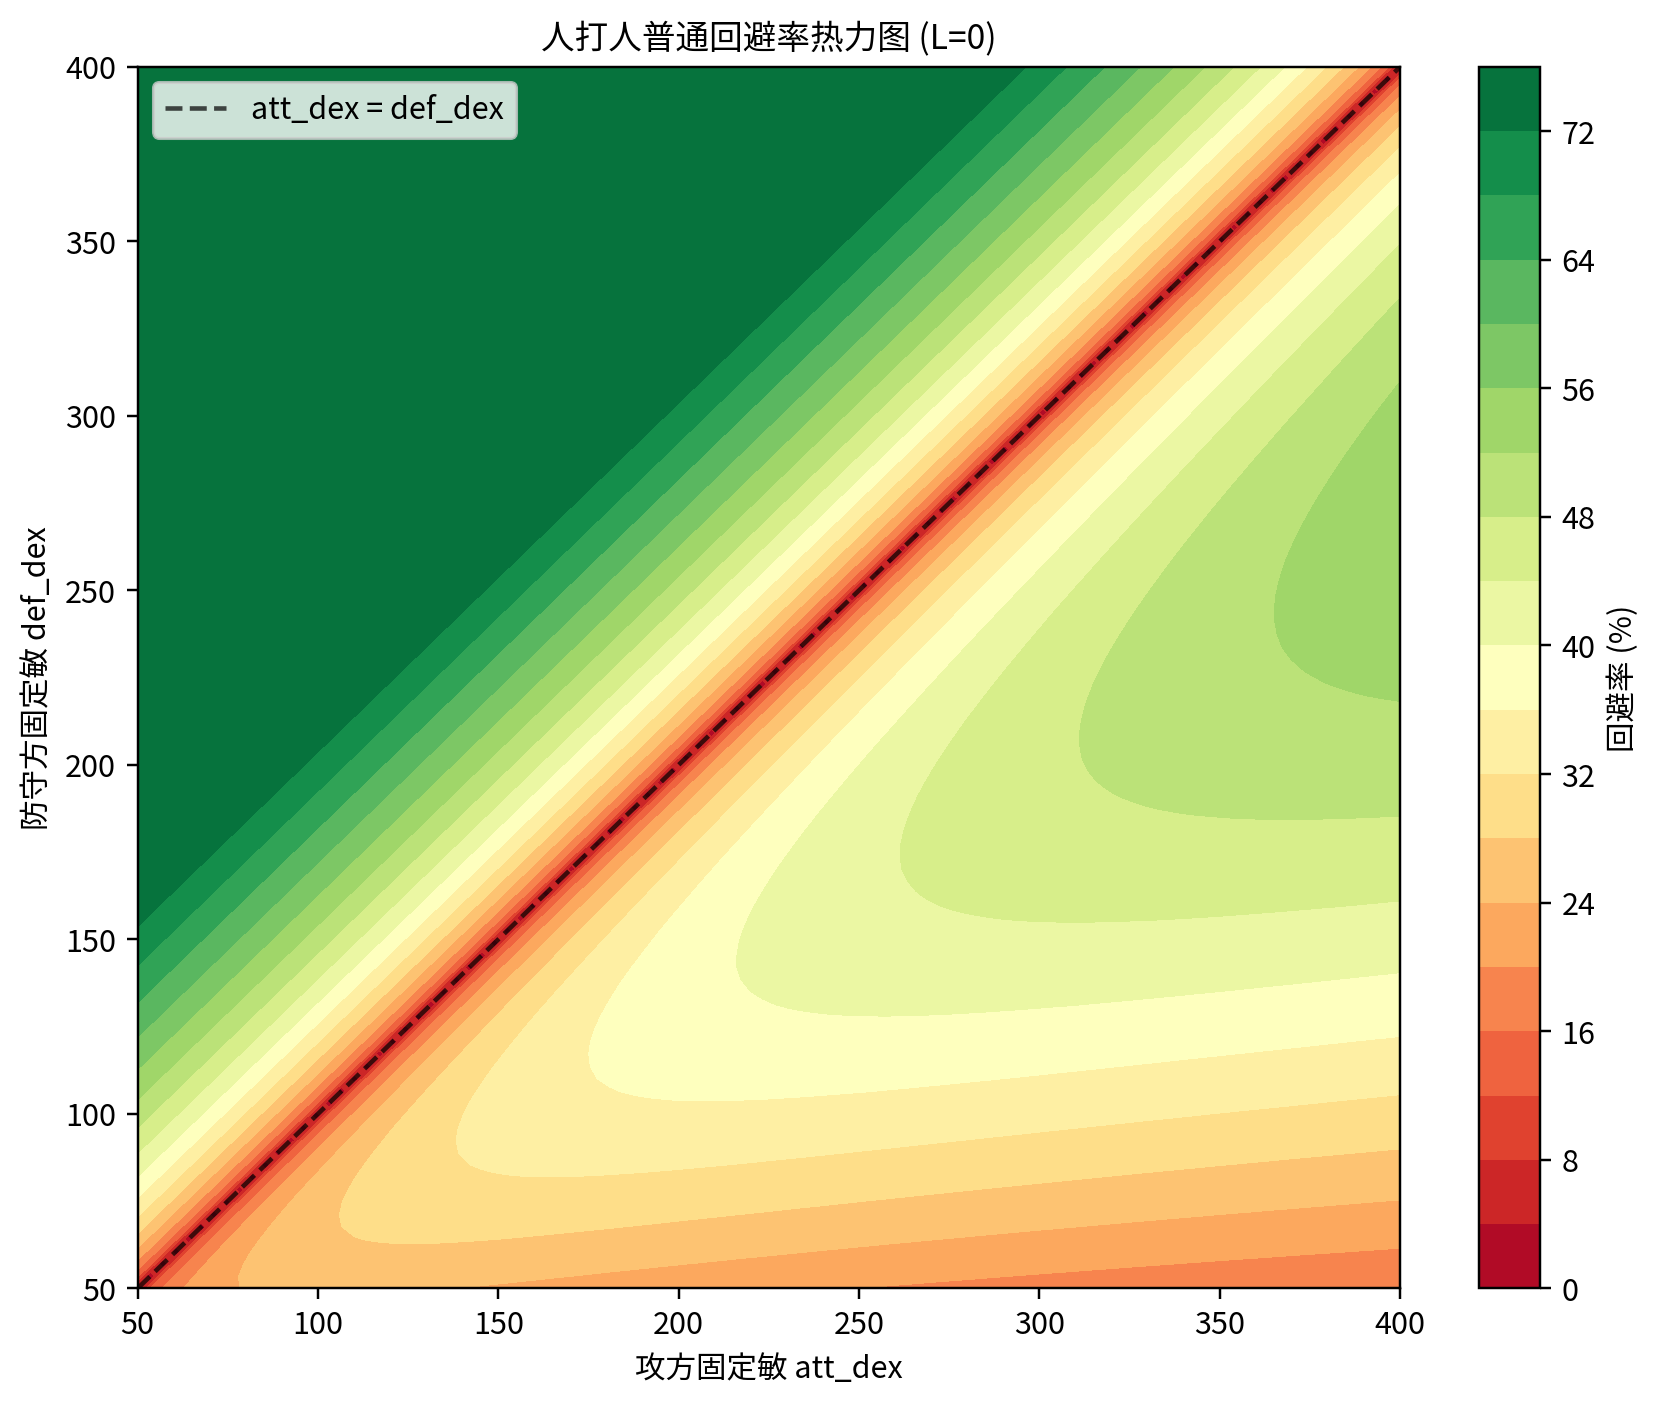
\includegraphics[width=0.75\textwidth]{figures/dodge_heatmap.png}
\caption{人打人普通回避率热力图 ($L=0$)}
\label{fig:dodge-heatmap}
\end{figure}

\begin{figure}[H]
\centering
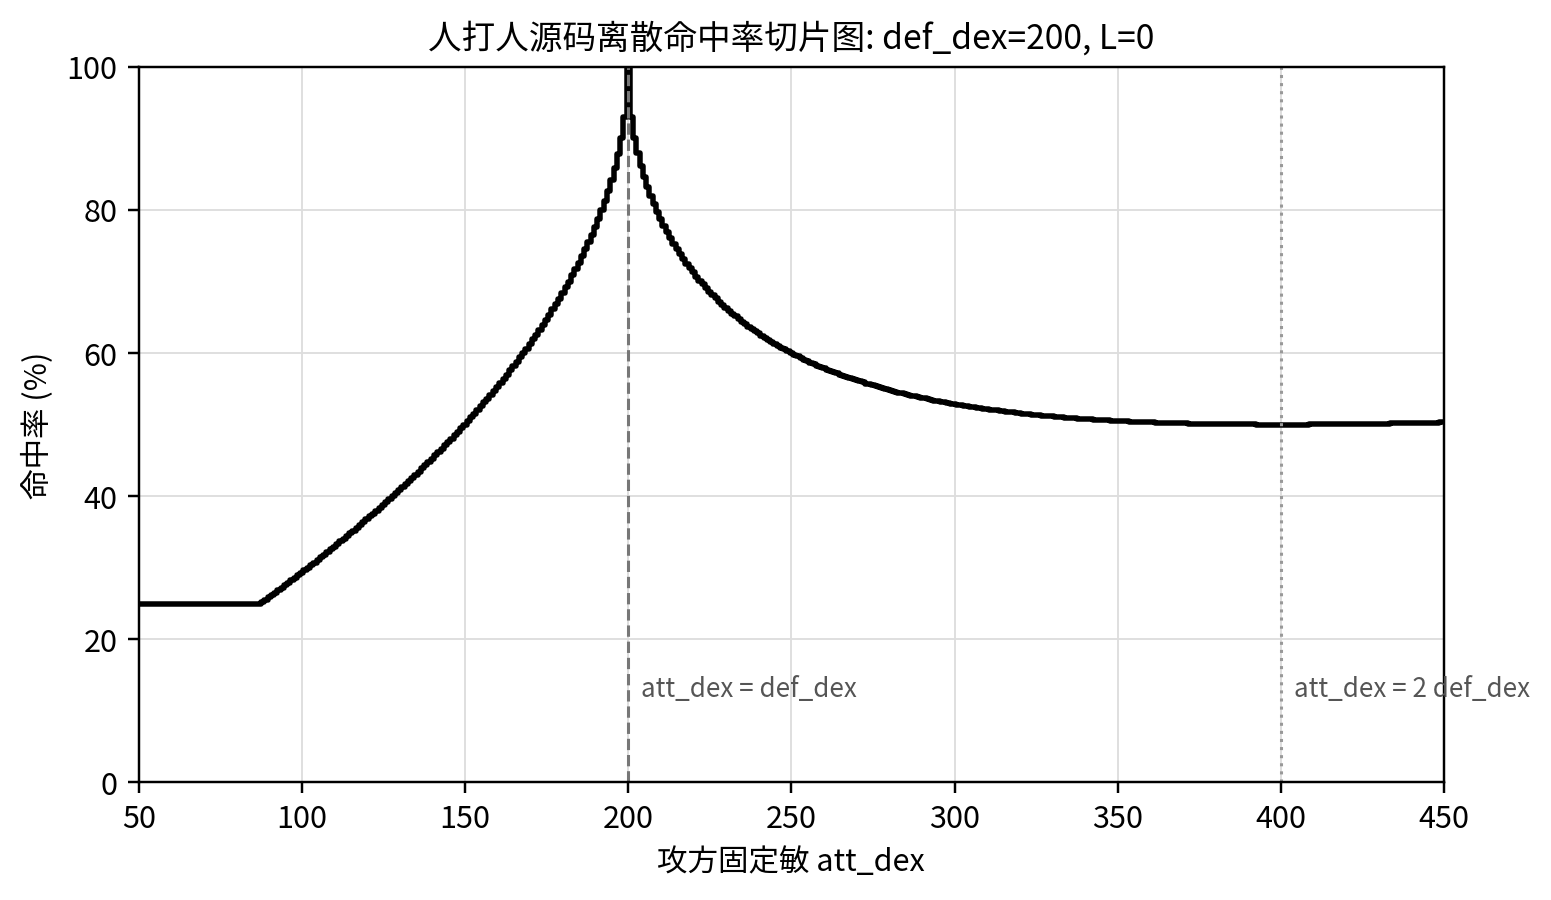
\includegraphics[width=0.75\textwidth]{figures/hit_slice_y200.png}
\caption{人打人命中率切片图 ($\defdex=200, L=0$)}
\label{fig:hit-slice}
\end{figure}

\subsection{实战上最容易写错的细节}

这一段源码里有四个非常容易被简化过头的细节。其一，身份修正不是“攻守两边都按同一规则缩放”，而是按对象组合只修一边。其二，弓修正会在普通回避流程中加两次。其三，\code{AddHit} 发生在 $[1,7500]$ 裁切之后，而职业技能 \textbf{回避} 的倍率又发生在 \code{AddHit} 之后。其四，混乱攻击会在这些步骤之后再把当前回避值提高 $40\%$。这几个步骤的相对顺序不能交换，否则就会得到与源码不同的边界结果。

\section{会心公式与武器会心}

\subsection{源码顺序与身份修正}

会心判定与回避不同，并不共享同一套身份修正规则。设攻击方与防守方原始固定敏仍为 $\attdex$ 与 $\defdex$，武器会心值为 $C$，攻击方幸运为 $L_a$。在当前主分支下，会心公式的身份修正可整理为
\begin{equation}
    (\widehat{\attdex},\widehat{\defdex},\beta,\rho)=
    \begin{cases}
        (\attdex,\lfloor 0.8\defdex \rfloor,0.09,\sqrt{\cdot}), & \text{宠物打敌人}, \\
        (\attdex,\defdex,10,\mathrm{id}), & \text{敌人打宠物}, \\
        (\attdex,\defdex,10,\mathrm{id}), & \text{非玩家打玩家}, \\
        (\attdex,\lfloor 0.6\defdex \rfloor,0.09,\sqrt{\cdot}), & \text{玩家打非玩家}, \\
        (\attdex,\defdex,0.09,\sqrt{\cdot}), & \text{其余情形}.
    \end{cases}
\end{equation}
其中 $\rho$ 记号用来区分“平方根口径”和“线性口径”：若 $\rho=\sqrt{\cdot}$，源码取平方根；若 $\rho=\mathrm{id}$，则直接取一次差值，不再开根。

令
\begin{equation}
    B = \max\{\widehat{\attdex},\widehat{\defdex}\}, \qquad S = \min\{\widehat{\attdex},\widehat{\defdex}\},
\end{equation}
并定义
\begin{equation}
    w = \begin{cases}
        1, & \widehat{\attdex} \ge \widehat{\defdex}, \\
        \dfrac{\widehat{\attdex}}{\widehat{\defdex}}, & \widehat{\attdex} < \widehat{\defdex}.
    \end{cases}
\end{equation}
则会心基础体为
\begin{equation}
    c_{\mathrm{core}} =
    \begin{cases}
        \sqrt{\max\!\left\{\dfrac{B-S}{\beta},0\right\}} + 0.5C, & \rho=\sqrt{\cdot}, \\
        \max\!\left\{\dfrac{B-S}{\beta},0\right\} + 0.5C, & \rho=\mathrm{id},
    \end{cases}
\end{equation}
\begin{equation}
    c_{\mathrm{raw}} = c_{\mathrm{core}}\,w + L_a.
\end{equation}
源码随后执行
\begin{equation}
    c_{\mathrm{work}} = \min\!\left\{10000,\max\!\left\{1,\left\lfloor 100c_{\mathrm{raw}}\right\rfloor\right\}\right\},
\end{equation}
并以 \code{RAND(1,10000) < c\_work} 判定是否会心成立。

\subsection{玩家打玩家的离散化简式}

对玩家 PVP 而言，上述身份修正退化为 $\widehat{\attdex}=\attdex$、$\widehat{\defdex}=\defdex$、$\beta=0.09$ 且采用平方根口径，于是连续基础体可写为
\begin{equation}
    c_{\mathrm{base}}(\attdex,\defdex,L,C)=
    \begin{cases}
        \sqrt{\dfrac{\attdex-\defdex}{0.09}}+L+0.5C, & \attdex \ge \defdex, \\
        \left(\sqrt{\dfrac{\defdex-\attdex}{0.09}}+0.5C\right)\dfrac{\attdex}{\defdex}+L, & \attdex < \defdex.
    \end{cases}
    \label{eq:crit-base}
\end{equation}
对应的源码离散化会心率为
\begin{equation}
    p_{\mathrm{crit}}^{\mathrm{src}}(\attdex,\defdex,L,C)
    = 0.01\min\!\left\{9999,\max\!\left\{0,\left\lfloor 100c_{\mathrm{base}}(\attdex,\defdex,L,C)\right\rfloor-1\right\}\right\}.
    \label{eq:crit-final}
\end{equation}
之所以是减去 $1$，是因为源码最终使用的是严格小于号 \code{<}，而不是回避公式中的小于等于号 \code{<=}。

另一个非常容易被误解的点是弓。当前实现中，弓并非“不能会心”，而是“即使判出会心，也不走额外的会心伤害函数”。换言之，弓在概率意义上仍可产生会心事件，但该事件在伤害层面的收益会被显著削弱。

\section{反击触发条件、离散公式与次数上限}

\subsection{触发条件}

反击并不是一个无条件概率，而是一系列条件之后的后验事件。首先，当前出手动作必须属于可反击类型，当前主分支主要对应普通攻击与无防御攻击。其次，反击方和被反击方都必须存活。再次，带有本回合忠诚失控标记 \code{CHAR_BATTLEFLG_AIBAD} 的单位不能触发反击。最后，若任意一边使用的是弓、回力或投掷类远程武器，反击检查会直接失败。

源码主循环还显式限制了反击链的最大往返次数，因此反击不是无限触发过程，而是一个带有深度上限的离散链式事件。

\subsection{玩家打玩家时的反击离散化简式}

设反击方与被反击方固定敏分别为 $\attdex$ 与 $\defdex$。反击基础敏捷体与会心类似，但不带武器会心项。对玩家 PVP 简化口径，有
\begin{equation}
    q_{\mathrm{base}}(\attdex,\defdex)=
    \begin{cases}
        \sqrt{\dfrac{\attdex-\defdex}{0.08}}, & \attdex \ge \defdex, \\
        \sqrt{\dfrac{\defdex-\attdex}{0.08}}\dfrac{\attdex}{\defdex}, & \attdex < \defdex.
    \end{cases}
    \label{eq:counter-base}
\end{equation}
记武器对武器系数为 $F$，反击方幸运为 $L$。若忽略 \code{_SUIT\_ADDENDUM} 下的额外反击修正，则源码中的玩家反击工作值可写成
\begin{equation}
    r_{\mathrm{counter}} = 0.1F\,q_{\mathrm{base}}(\attdex,\defdex)+L.
\end{equation}
最终的源码离散化反击率为
\begin{equation}
    p_{\mathrm{counter}}^{\mathrm{src}}(\attdex,\defdex,L,F)
    = 0.01\min\!\left\{10000,\max\!\left\{0,\left\lceil 100r_{\mathrm{counter}}\right\rceil-1\right\}\right\}.
    \label{eq:counter-final}
\end{equation}
这里之所以出现上取整与减去 $1$，正是因为源码最终比较的是 \code{RAND(1,10000) < 100*r\_counter}。若讨论宠物反击，则还要额外加入 \code{BATTLE\_COM\_S\_NOGUARD} 的附加值，并注意宠物分支会在进入随机判定前显式裁切到 $100\%$。

\section{变量影响分析与单调性讨论}

以下讨论只针对“人打人”这条玩家 PVP 支路的\emph{连续化主体}，即暂时忽略回避、会心、反击公式中的取整、上下限裁切，以及严格小于或小于等于带来的 $0.01\%$ 级偏移。这样做的目的不是替代源码，而是把源码离散结果背后的主导趋势提取出来。

\subsection{命中对攻方敏捷并非全局单调}

先把式~\eqref{eq:dodge-final} 与式~\eqref{eq:hit-final} 中的取整与裁切去掉，只保留连续主体。此时命中率对攻方敏捷的导数满足：当 $\attdex<\defdex$ 时，
\begin{equation}
    \frac{\partial p_{\mathrm{hit}}}{\partial \attdex} = \frac{1}{2\sqrt{0.02}\sqrt{\defdex-\attdex}} > 0,
\end{equation}
因此攻方敏捷低于守方时，继续补敏一定提高命中。然而当 $\attdex>\defdex$ 时，
\begin{equation}
    \frac{\partial p_{\mathrm{hit}}}{\partial \attdex}
    = \frac{\defdex(\attdex-2\defdex)}{2\sqrt{0.02}\,\attdex^2\sqrt{\attdex-\defdex}}.
    \label{eq:hit-derivative}
\end{equation}
式~\eqref{eq:hit-derivative} 的符号取决于 $\attdex-2\defdex$，于是会出现三个区间：$\defdex<\attdex<2\defdex$ 时导数为负，$\attdex=2\defdex$ 时导数为零，$\attdex>2\defdex$ 时导数重新转正。也就是说，在“刚刚超过守方敏捷但还没到两倍”的区间里，继续堆攻方敏捷反而可能降低命中率。

\subsection{会心存在局部非单调区间}

对式~\eqref{eq:crit-base} 的连续主体，若先固定 $L$ 与 $C$，当 $\attdex>\defdex$ 时有
\begin{equation}
    \frac{\partial p_{\mathrm{crit}}}{\partial \attdex} = \frac{1}{2\sqrt{0.09}\sqrt{\attdex-\defdex}} > 0,
\end{equation}
因此攻方敏捷领先后，会心率单调上升。然而在 $\attdex<\defdex$ 且先忽略武器会心时，
\begin{equation}
    \frac{\partial p_{\mathrm{crit}}}{\partial \attdex} = \frac{2\defdex-3\attdex}{2\defdex\sqrt{0.09}\sqrt{\defdex-\attdex}}.
    \label{eq:crit-derivative}
\end{equation}
由式~\eqref{eq:crit-derivative} 可知，当 $\attdex<2\defdex/3$ 时，会心率随攻方敏捷增加而上升；当 $2\defdex/3<\attdex<\defdex$ 时，会心率反而下降。武器会心 $C$ 的存在会把这一拐点向右推移，但不能消除非单调结构本身。

\subsection{反击的主导单调性与会心同型}

对式~\eqref{eq:counter-final}，若暂时去掉上取整与边界裁切，只保留连续主体 $0.1F\,q_{\mathrm{base}}+L$，则当 $\attdex>\defdex$ 时有
\begin{equation}
    \frac{\partial p_{\mathrm{counter}}}{\partial \attdex}
    = \frac{F}{20\sqrt{0.08}\sqrt{\attdex-\defdex}} > 0.
\end{equation}
而在 $\attdex<\defdex$ 时，
\begin{equation}
    \frac{\partial p_{\mathrm{counter}}}{\partial \attdex}
    = \frac{F(2\defdex-3\attdex)}{20\defdex\sqrt{0.08}\sqrt{\defdex-\attdex}}.
    \label{eq:counter-derivative}
\end{equation}
因此，对固定正武器系数 $F$ 而言，反击在单调性上与“武器会心取 $0$ 的会心公式”完全同型：当 $\attdex<2\defdex/3$ 时先升，进入 $2\defdex/3<\attdex<\defdex$ 后转为下降，越过 $\attdex=\defdex$ 后重新单调上升。武器系数 $F$ 的作用主要是对整条曲线做比例缩放，而不是改变拐点位置。

\subsection{变量位置不同，收益性质就不同}

综合回避、会心与反击三条链可以看到：幸运、武器会心、武器对武器系数、\code{AddHit}、职业技能 \textbf{回避} 与混乱攻击修正，并不是在同一层进入公式。幸运大多表现为平移项；武器会心只作用于会心；武器对武器系数只作用于玩家反击；\code{AddHit} 发生在回避上限裁切之后；职业技能 \textbf{回避} 则发生在 \code{AddHit} 之后再做倍率放大。也正因为如此，石器时代里“每加一点某属性的收益”并不是统一线性的概念，而必须放回变量真正进入判定链的位置来讨论。

\section{源码离散值表与切片图}

图~\ref{fig:hit-crit-table} 与图~\ref{fig:hit-crit-slices} 都只画“人打人”这条支路。具体地，固定守方敏捷为 $\defdex=200$，并统一取守方幸运 $L_d=0$、攻方幸运 $L_a=0$、武器会心值 $C=0$、玩家反击武器系数 $F=10$，同时忽略弓、醉酒、\code{AddHit}、职业技能 \textbf{回避}、无防御攻击附加与混乱攻击修正。表中给出的命中率、会心率与反击率，均按本章的源码离散化简式直接计算，而不是用连续近似值代替。

\begin{figure}[H]
    \centering
    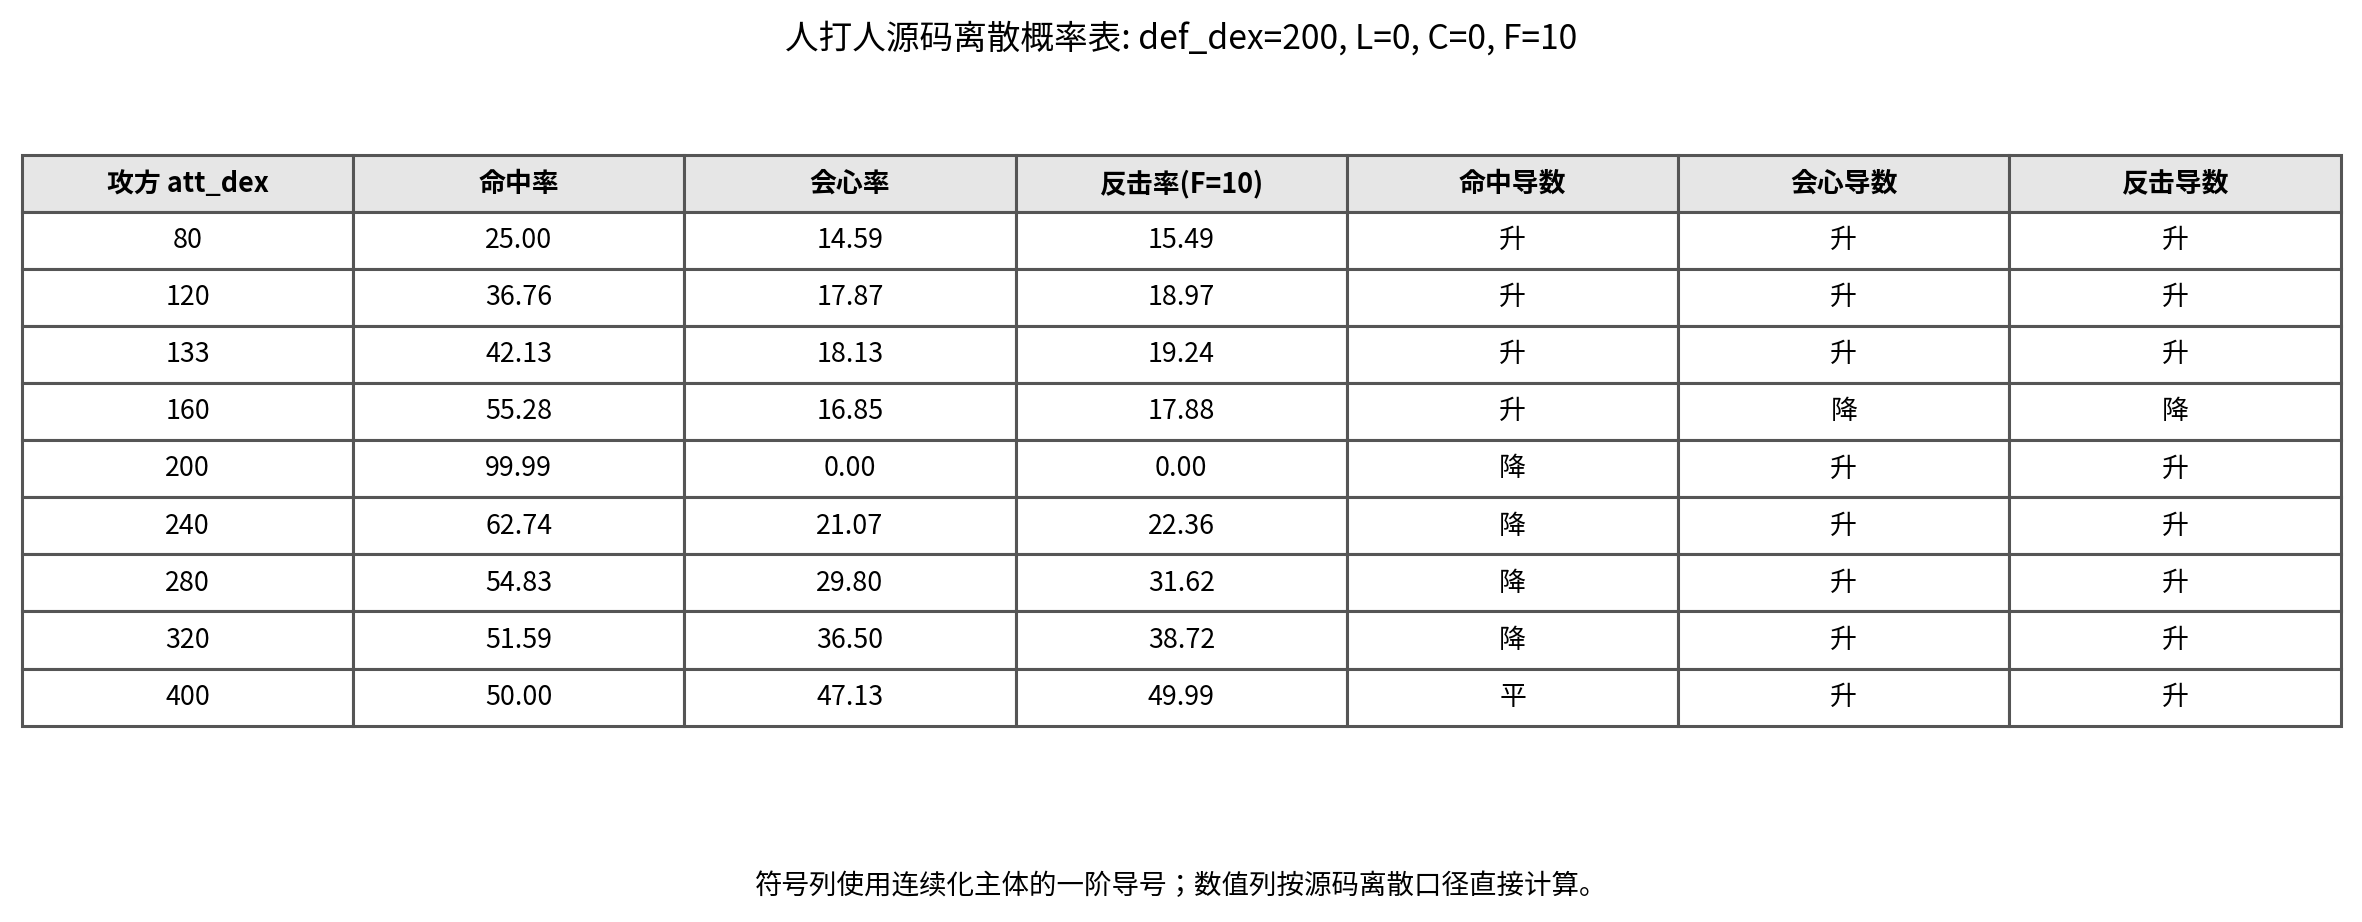
\includegraphics[width=0.9\textwidth]{figures/hit_crit_table_y200.png}
    \caption{固定守方敏捷 $\defdex=200$ 时的源码离散概率表。统一取 $L_d=L_a=0$、$C=0$、$F=10$，并关闭弓、醉酒、\code{AddHit}、职业技能 \textbf{回避}、无防御攻击附加与混乱攻击修正。表中符号列使用连续化主体的一阶导号，只用于展示主导趋势。}
    \label{fig:hit-crit-table}
\end{figure}

图~\ref{fig:hit-crit-slices} 进一步给出同一组参数下的切片图。三张图中的曲线都来自源码离散化简式，因此会呈现出台阶状；而虚线和点线标记的则是连续化主体中的关键阈值，用于说明“源码离散结果”和“连续趋势分析”之间是如何对应的。

\begin{figure}[H]
    \centering
    \begin{subfigure}[b]{0.48\textwidth}
        \centering
        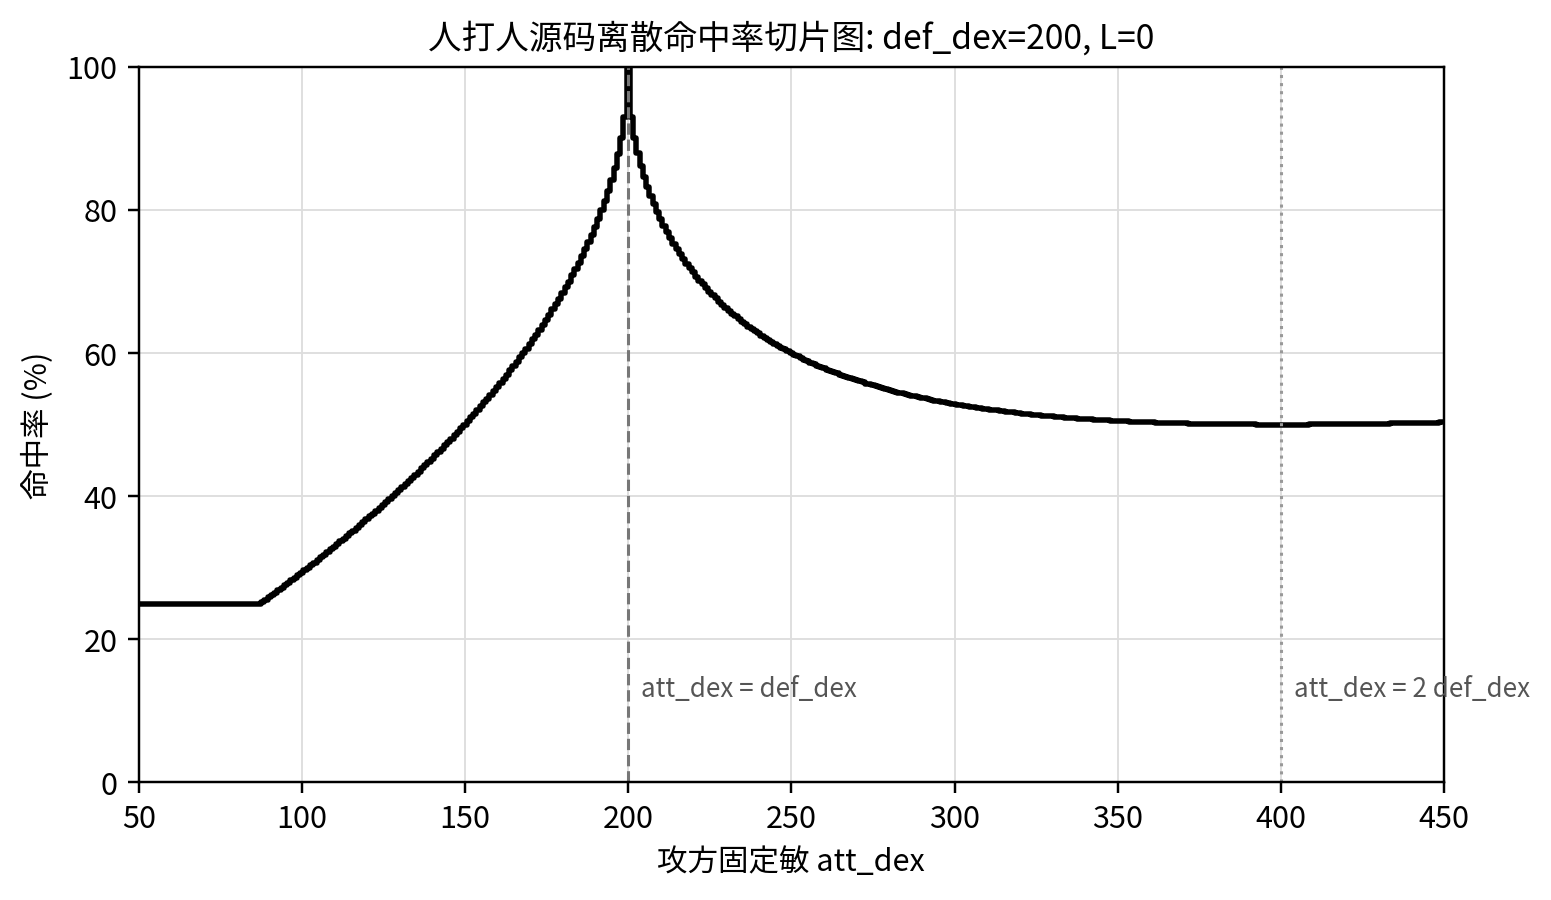
\includegraphics[width=\textwidth]{figures/hit_slice_y200.png}
        \caption{命中率切片图}
    \end{subfigure}
    \hfill
    \begin{subfigure}[b]{0.48\textwidth}
        \centering
        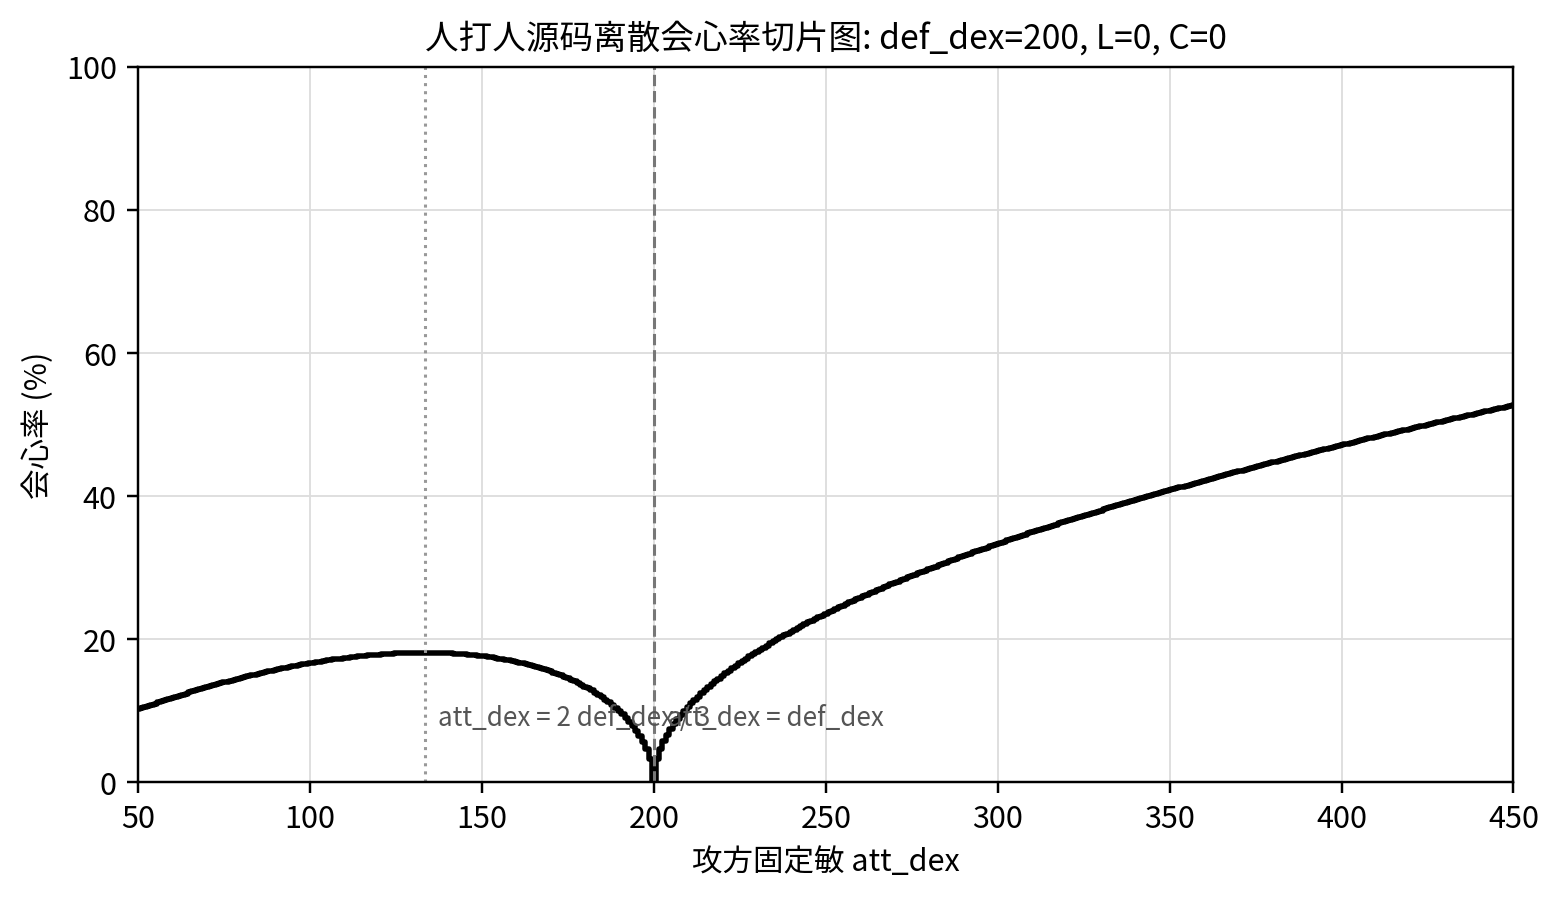
\includegraphics[width=\textwidth]{figures/crit_slice_y200.png}
        \caption{会心率切片图}
    \end{subfigure}

    \medskip
    \begin{subfigure}[b]{0.66\textwidth}
        \centering
        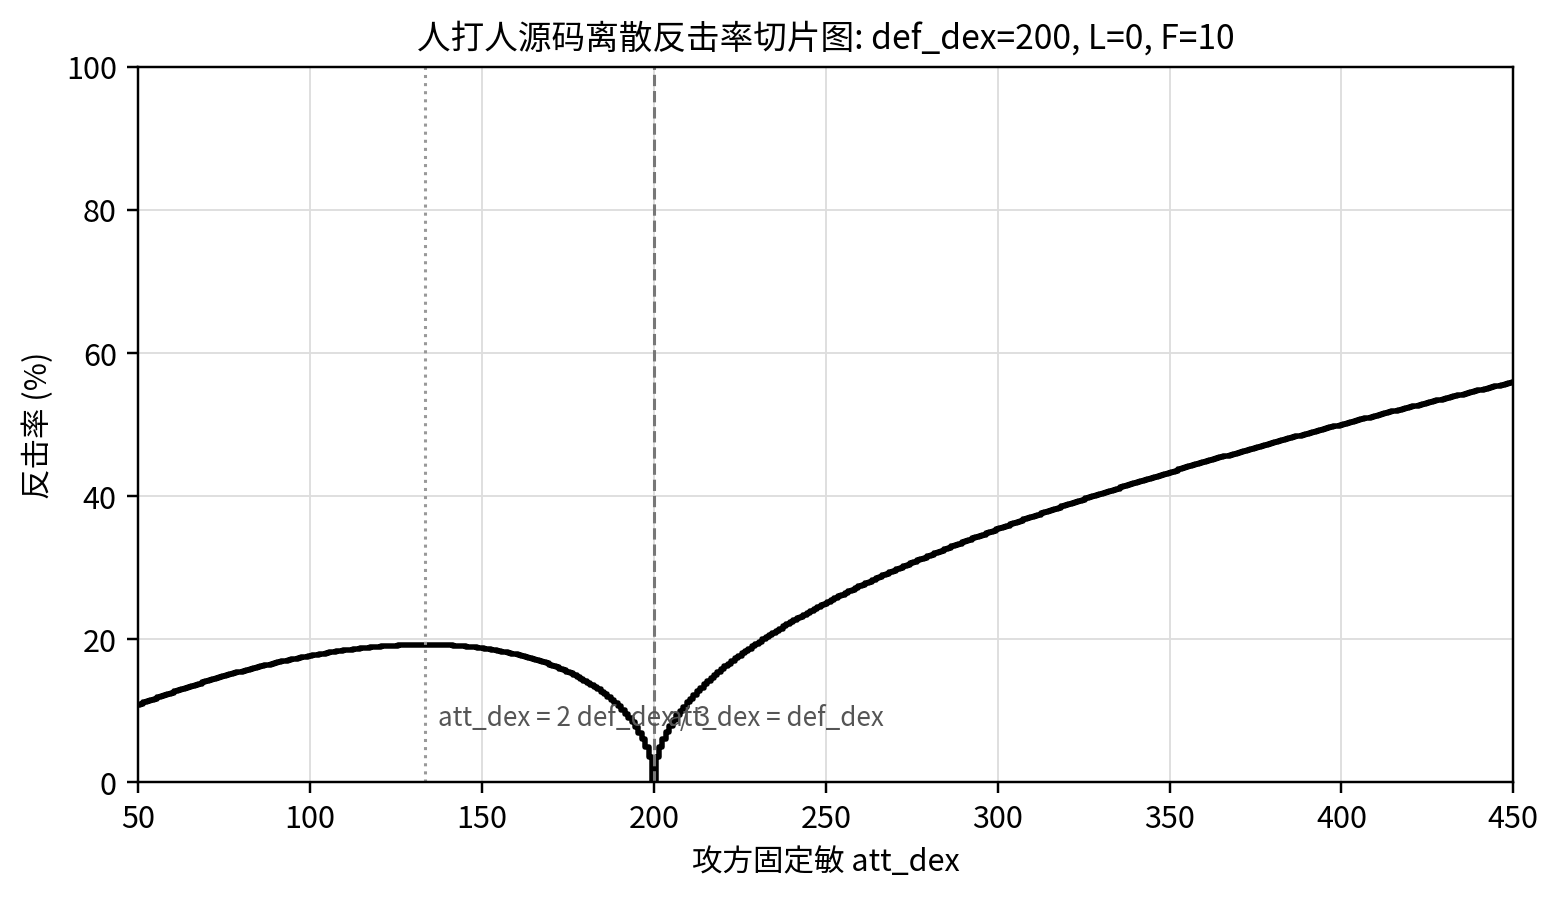
\includegraphics[width=\textwidth]{figures/counter_slice_y200_f10.png}
        \caption{反击率切片图（$F=10$）}
    \end{subfigure}
    \caption{玩家 PVP 简化口径下的源码离散切片图。统一取守方固定敏 $\defdex=200$、幸运为 $0$；会心图额外取武器会心值 $C=0$，反击图额外取武器系数 $F=10$。图中的阈值线来自连续化主体，用于标记导数符号发生变化的位置。}
    \label{fig:hit-crit-slices}
\end{figure}

从这些图可以直接看到：命中率在 $\defdex<\attdex<2\defdex$ 区间出现局部下降；会心率和反击率则都在 $2\defdex/3<\attdex<\defdex$ 区间出现局部下降。也就是说，源码中的非单调性并不是推导技巧造成的假象，而是离散数值表里可以直接观察到的结构事实。